
\subsection{Red de una empresa}
Este experimento sobre una red Wi-Fi en una empresa con alrededor de 15 empleados. En esta red se suelen conectar varios dispositivos moviles y también notebooks.

\subsubsection{Fuente S}

Utilizando las herramientas presentadas en el ejercicio 1 sobre esta red se obtuvieron los siguientes resultados
\begin{itemize}
 \item $12039$ paquetes unicasts
 \item $6561$ paquetes broadcasts
 \item $18600$ paquetes en total
\end{itemize}

 La \emph{entrop\'ia} para esta fuente se calcul\'o en  $0.936493026389$. El siguiente grafico muestra este comportamiento. \par
 %\textbf{METER EL GRAFIQUITO DE LA ENTROPIA UNICAST Y BROADCAST}

%\blindtext

\begin{figure}[h]
   \centering
   \begin{tabular}{@{}c@{\hspace{.5cm}}c@{}}
       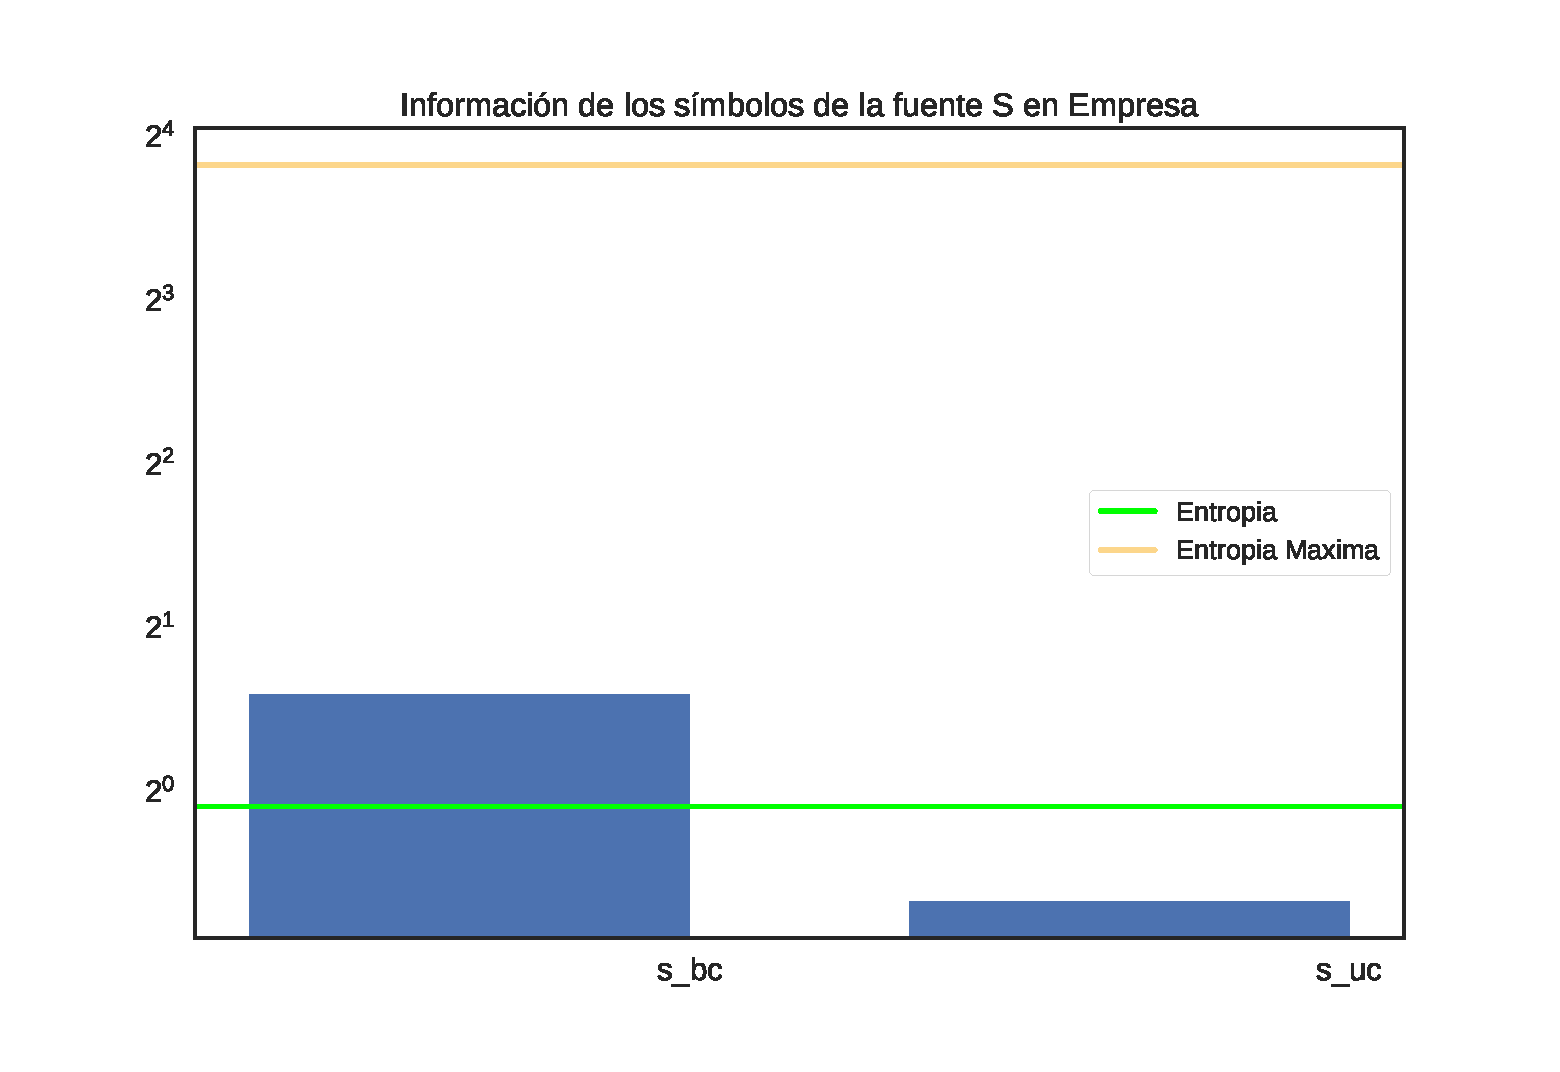
\includegraphics[page=1,width=.70\textwidth]{../img/barras-Empresa} &
       %\includegraphics[page=2,width=.45\textwidth]{somemultipagepdf} \\[.5cm]
       %\includegraphics[page=3,width=.45\textwidth]{somemultipagepdf} \\
   \end{tabular}
 \caption{Entrop\'ia de la red}
 \label{fig:Test}
\end{figure}

%\blindtext




 Como la medici\'on se realiza sobre una red inalambrica a la cual se encuentran conectados varios dispositivos, es razonable que exista una mayor presencia de paquetes \emph{unicast}. Esto es porque dichos dispositivos, generalmente, envian paquetes a un destino IP particular con la finalidad de conectarse a alg\'un servidor externo. \par


 \subsubsection{Grafo de conectividad de la red}
 Grafo de conectividad de la red para visualizar el comportamiento de la misma.


\begin{figure}[h]
   \centering
   \begin{tabular}{@{}c@{\hspace{.5cm}}c@{}}
       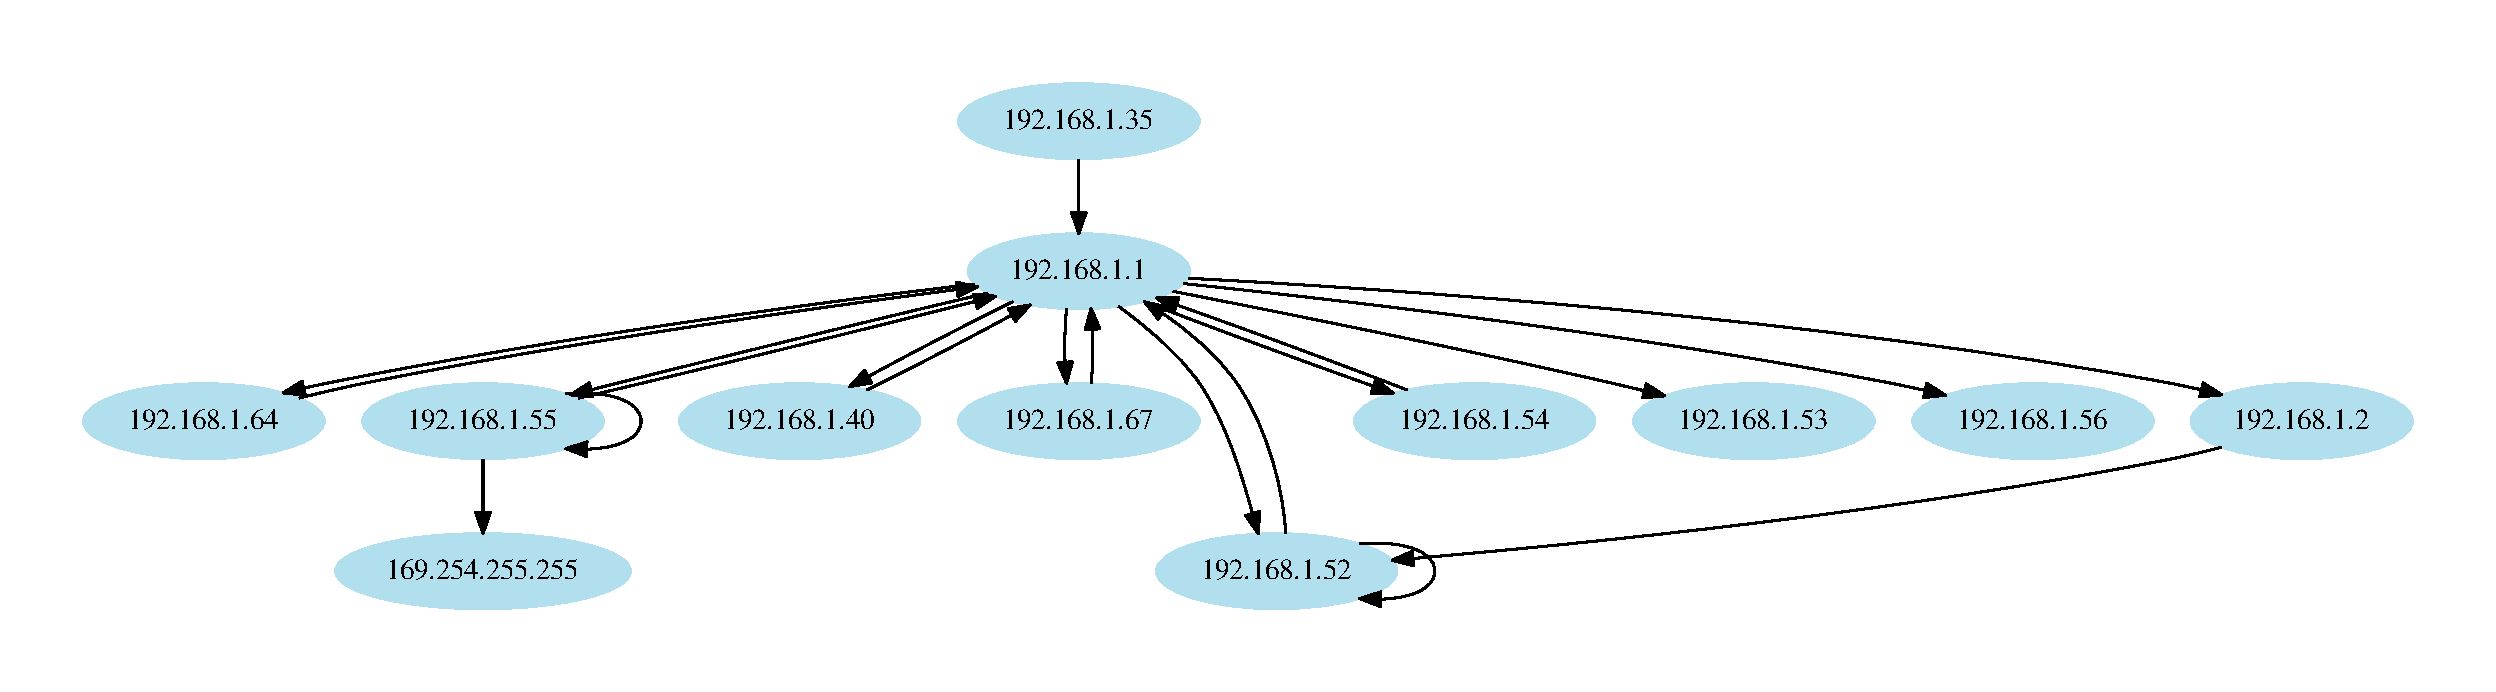
\includegraphics[page=1,height=8cm ,width=1.08\textwidth]{../img/red-Empresa} &
       %\includegraphics[page=2,width=.45\textwidth]{somemultipagepdf} \\[.5cm]
       %\includegraphics[page=3,width=.45\textwidth]{somemultipagepdf} \\
   \end{tabular}
 \caption{Grafo de conectividad}
 \label{fig:Test}
\end{figure}

% \textbf{GRAFICO!!}

 En la figura anterior se puede observar que el nodo 192.168.1.1 se comporta como un nodo raiz al cual se conectan varios dispositivos, este comportamiento es esperado debido a que se trata de una red Wi-Fi en el cual el nodo 192.168.1.1 podr\'ia el Router. \\

 A su vez, se puede observar que las direcciones asignadas son de la forma 192.168.1.0 con una m\'ascara $/25$ ya que ninguno de los \emph{hosts} tiene asignado direcciones superiores a $126$. \\

Tambi\'en se puede observar un pedido de asignaci\'on de IP por parte del host 192.168.1.55 hacia el servidor DHCP (169.254.255.255).\\

Por \'ultimo podemos observar paquetes en las cuales la direcci\'on de destino coincide con la direcci\'on del emisor, esto se debe a que son \emph{gratuitous ARP packets} los cuales suponemos son utilizados para anunciar a la red de la presencia de un nuevo dispositivo o para actualizar las tablas de ARP luego de que una MAC address cambia de IP.


 \subsubsection{Informacion y nodos distingidos}
 Para esta secci\'on reutilizamos la herramienta presentada en el ejercicio 2 con el objetivo de analizar la presencia de nodos distinguidos de la fuente. \\

 Como se puede observar en la figura \ref{fig:Test}, el dispositivo 192.168.1.1 se comporta como \'unico nodo distinguido de nuestra red y su direcci\'on se corresponde con las asignadas generalmente por los Routers, por este motivo no es precipitado suponer que podr\'ia tratarse del \emph{default gateway} de esta red.

\begin{figure}[H]
   \centering
   \begin{tabular}{@{}c@{\hspace{   .5cm}}c@{}}
       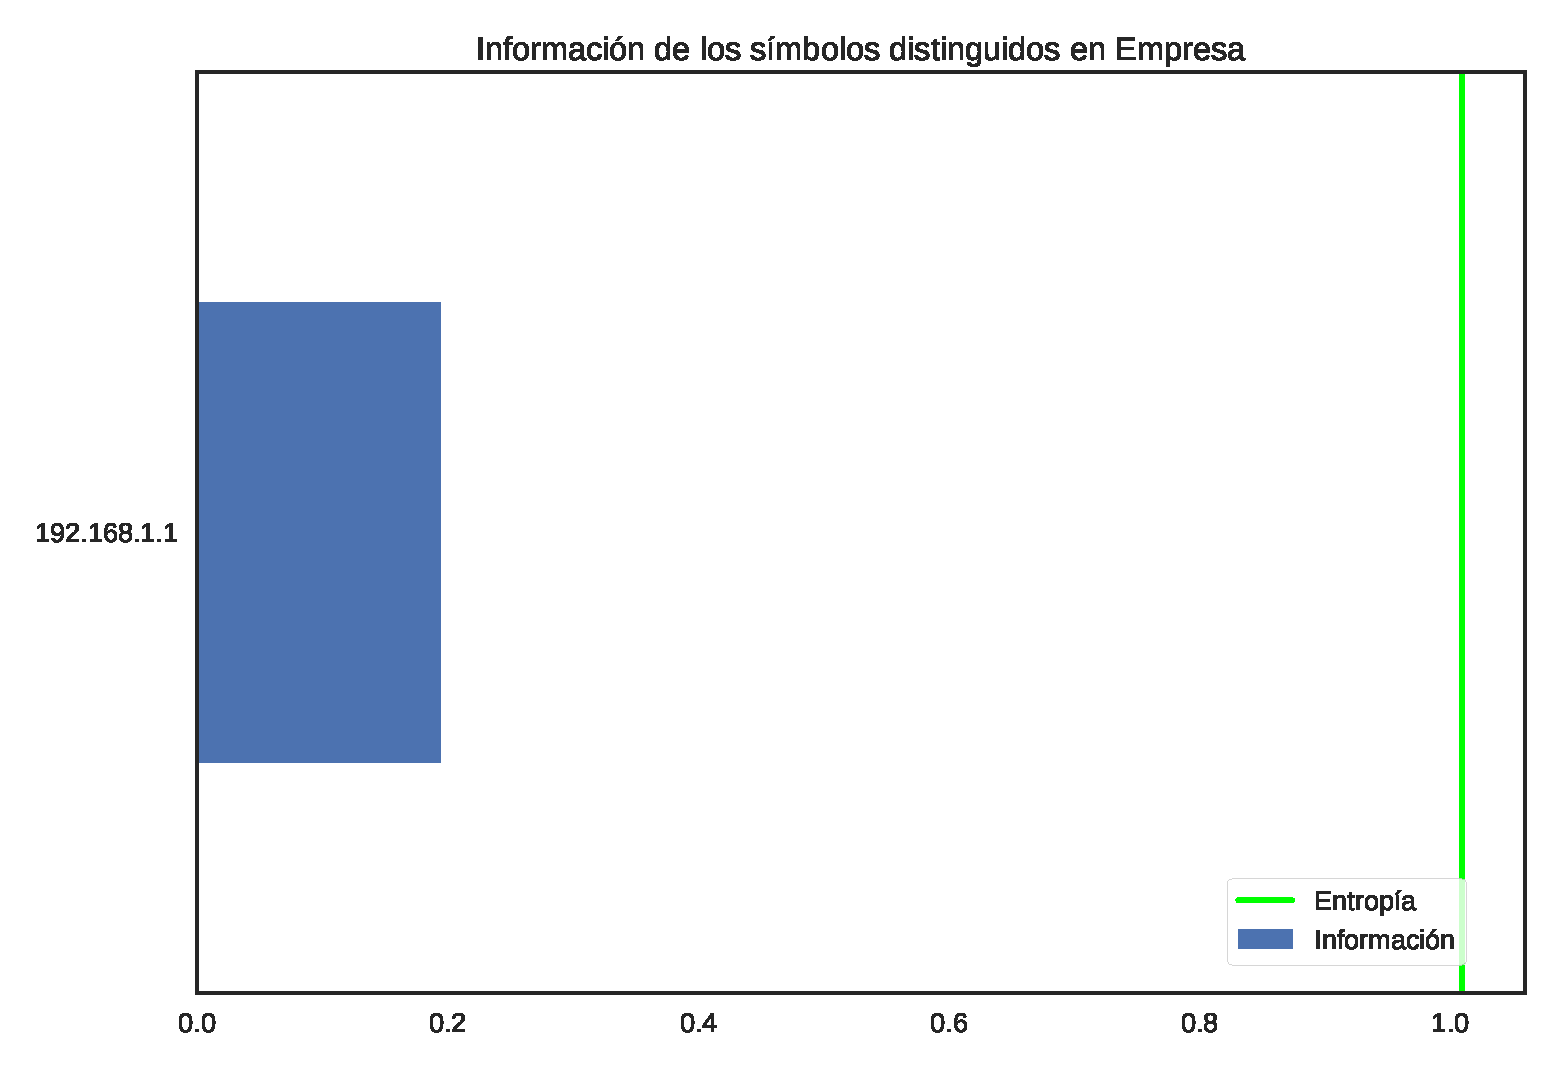
\includegraphics[page=1, height=6.8cm ,width=\textwidth]{../img/distinguidos-Empresa} &
       %\includegraphics[page=2,width=.45\textwidth]{somemultipagepdf} \\[.5cm]
       %\includegraphics[page=3,width=.45\textwidth]{somemultipagepdf} \\
   \end{tabular}
 \caption{Nodos distinguidos}
 \label{fig:Test}
\end{figure}


% \textbf{GRAFQUITO DEL NODO DISTINGUIDO}
